\documentclass[12pt]{article}

\usepackage{geometry}
\geometry{a4paper}
\geometry{margin=2.5cm,top=2cm,bottom=2cm}

\usepackage{lastpage}
\usepackage{fancyhdr}
\pagestyle{fancy}
\renewcommand{\headrulewidth}{0.4pt}
\renewcommand{\footrulewidth}{0.4pt}
\renewcommand{\sectionmark}[1]{ \markright{#1}{} }
\lhead{Cyril NOVEL (cbn13)}\chead{}\rhead{\textit{ \nouppercase{\rightmark}}}
\lfoot{}\cfoot{\thepage\ of \pageref{LastPage}}\rfoot{}

\setlength{\headheight}{15pt}


\usepackage[english]{babel}
\usepackage[utf8]{inputenc}
\usepackage{amsmath}
\usepackage{graphicx}
\usepackage{algpseudocode}
\usepackage{algorithm}
\usepackage{amsthm}
\usepackage{amssymb}
\usepackage{mathtools}
\usepackage{commath}
\usepackage{stmaryrd}

\title{OFusion\\
\large{CO542 Individual Project}}

\author{Cyril NOVEL}

\date{\today}

\begin{document}
\maketitle
\newpage

\tableofcontents

\newpage

\addcontentsline{toc}{section}{Introduction}
\section*{Introduction}

\newpage

\section{Hardware review}
\subsection{Virtual reality headsets}
A virtual reality headsets is a device capable of displaying 3D scenes to the user wearing the headset. It is made of screen and two lenses, with the left part of the screen showing the image for the left eye and the right eye for the right part.

Virtual reality headsets have been fancied a long-time and are finally becoming reality. The Oculus Rift is the first affordable headset to encounter a commercial success. Previously, Nintendo tried to sell a virtual reality headset called the Virtual Boy. It was a failure since its use caused terrible headaches to the players and only 5 shades of red were available.

In the following sections, we will present some virtual reality headsets and highlight their differences.

\subsubsection{Oculus Rift and Sony Morpheus}
The Oculus Rift is developped by Oculus VR. It is the first virtual headset targetting the mass market, and therefore has an aggressive price -- the first development kit costs 300\$, 350\$ for the second one.

The Oculus uses a screen for displaying the image. In the first development kit, the resolution of the screen was 1280x800, leading to an effective 640x800 per eye. One part of the screen displays the image for one eye, the other part displays the image for the other eye. The Rift uses lenses to distort the image on the screen, so that it fits the actual field of view of the human eye. The field of view of the Rift is 90 degrees horizontally. Figure~\ref{oculusback} shows the back of the Oculus Rift.

Gyros, accelerometers and magnetometers are combined in the helmet in order to track the user's head movements. The first development kit is however unable to detect translation movement.

\begin{figure}[h]
  \centering
  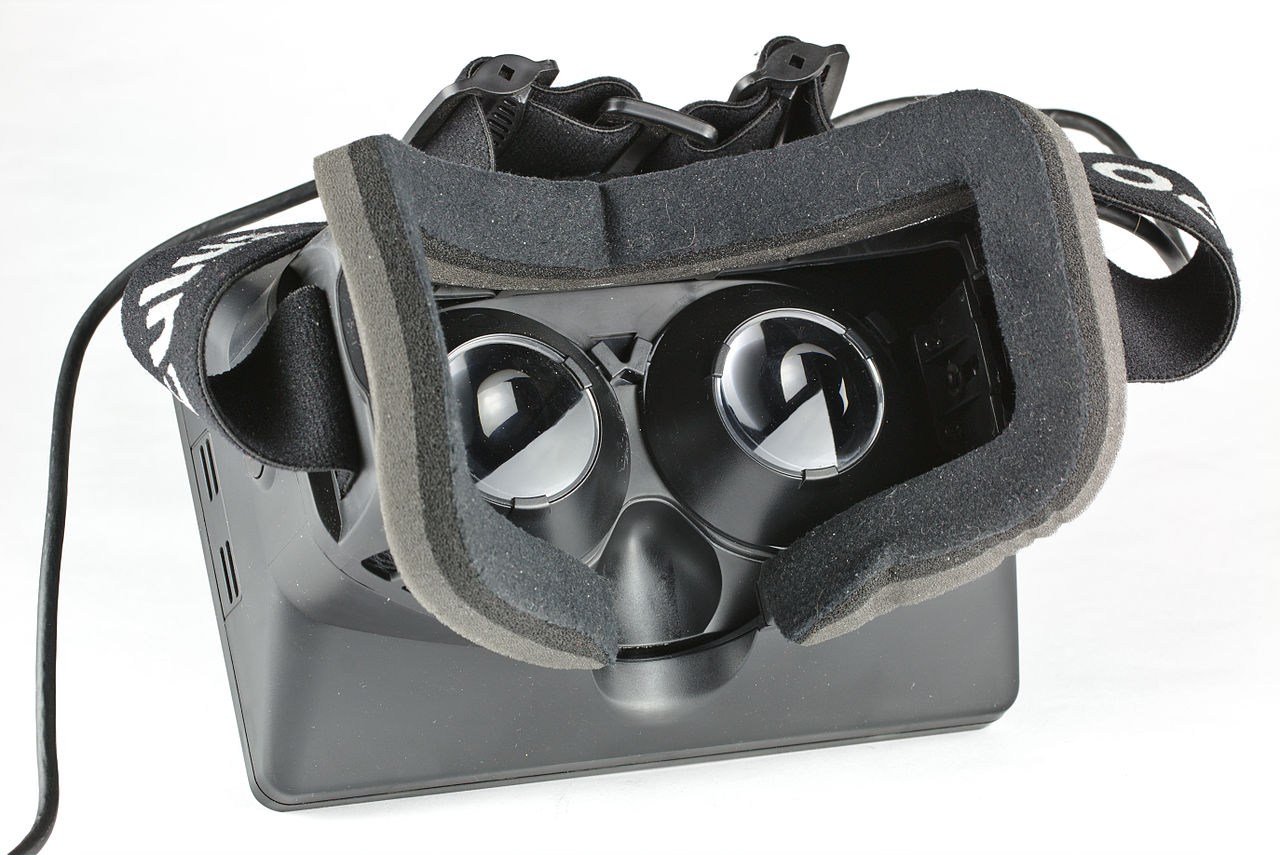
\includegraphics[scale=0.3]{OculusBack.jpg}
  \caption{\label{oculusback} The Oculus Rift}
\end{figure}

The major drawback of the Rift is the resolution of the screen. The screen-door effect is predominant and prevent a total immersion in the displayed scene. The second version of the Development Kit comes with a resolution of 960x1080 per eye, decreasing this effect. This next version comes also with a camera, tracking the movement of the head, in order to detect translation in addition to rotation.

The success of the Oculus Rift leads other companies to develop similar devices. Sony presented few weeks ago the project Morpheus -- shown in figure~\ref{morpheus}, highly similar to the Oculus Rift.

\begin{figure}[h]
  \centering
  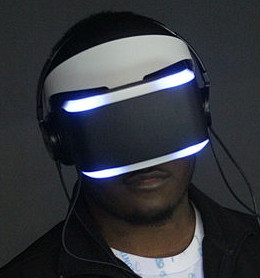
\includegraphics[scale=0.3]{Morpheus.jpg}
  \caption{\label{morpheus} Sony Morpheus}
\end{figure}

Sony Morpheus uses a comparable technology to Oculus Rift. The most noticable difference is that Morpheus has tracking technology all around it, whereas Oculus Rift only has tracking captors on the front and on the sides of the display.

\subsubsection{Google Cardboard and Samsung Gear VR}
During the Google I/O 2014, Google introduced the Cardboard Project. The idea is to use a smartphone as the screen for the headset and create the headset from a cardboard. Google presented the project as a Do-It-Yourself headset, acknowledging that the most difficult part was purchasing the lenses. The design files are available online and some online stores sell and ship the set for 25\$.

The advantage of Google Carboard is that it uses the sensors in the smartphone for the head positionning. Every recent smartphone is equiped with a gyroscope and a magnetometer

\subsubsection{Vrvana Totem}
The Totem, developed by Vrvana, is similar to the Oculus Rift, except that two cameras are embedded on the front of the headset -- see figure~\ref{tpg}. The idea is that each camera captures the view of one eye.

\begin{figure}[h]
  \centering
  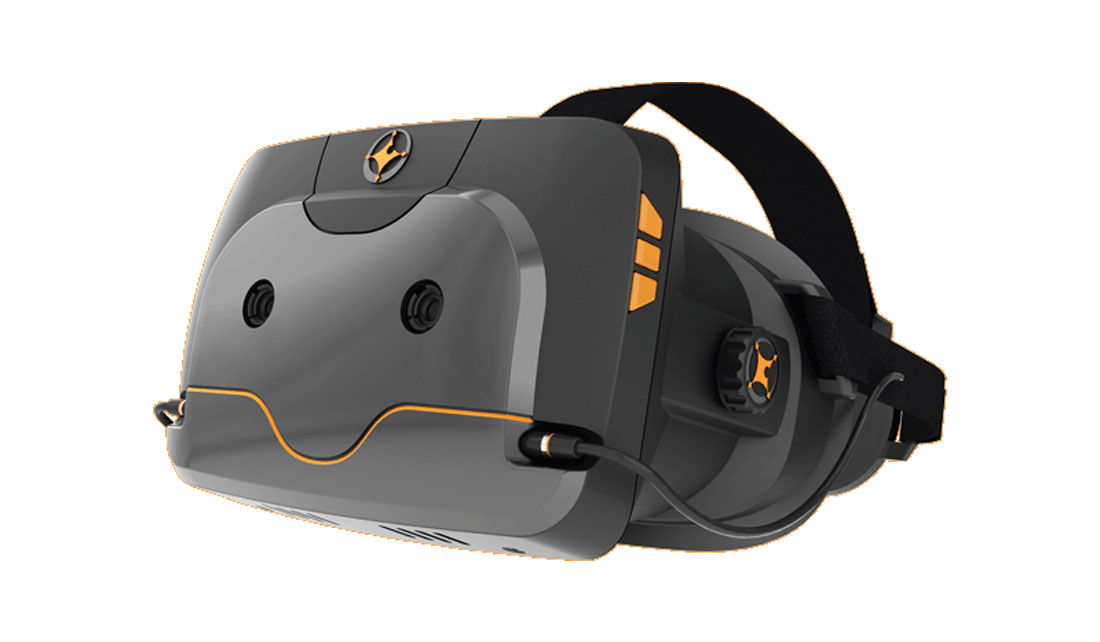
\includegraphics[scale=0.3]{TruePlayerGear.jpg}
  \caption{\label{tpg} The Totem, with two cameras}
\end{figure}

The lens distorsion is computed directly via the hardware in the headset. The others characteristics are higly similar to the Oculus Rift. The Totem is very interesting thanks to these embedded cameras. We want to achieve a new type of augmented reality. The Totem directly captures what the eyes would see.

\subsection{Test}
\label{subsec:pca}


\newpage
\section*{Conclusion}
\addcontentsline{toc}{section}{Conclusion}

\newpage
\addcontentsline{toc}{section}{References}
%\bibliographystyle{alpha}
%\bibliography{biblio}
\end{document}